\chapter{Technische Umsetzung}
\section{Beschreibung der App}
\subsection{Funktionen der jeweiligen Seiten}
\subsubsection{Homepage}
Die Homepage der App zeigt ein zufälliges und derzeit besonders beliebtes Spiel an, welches von der BoardGameGeek \ac{API} bezogen wird.
Die Generierung erfolgt automatisch und bei jedem Aufruf der Seite neu. Daher wird dieser Fähigkeit in der \texttt{ngOnInit()}-Funktion auf der Homepage aufgerufen.
Darüber hinaus dient die Homepage primär als Ausgangspunkt für die Navigation zu den anderen Seiten (siehe Tab. \ref{tab:homepage}).
\begin{table}[H]
    \centering
    \begin{tabular}{|c|c|}
        \hline
        \textbf{Funktion} & \textbf{Beschreibung} \\
        \hline
        \texttt{goToHomepage()} & Navigiere zur Homepage. \\
        \texttt{navigateToHome()} & Navigiere zur Homepage. \\
        \texttt{navigateToInventory()} & Navigiere zum Inventar. \\
        \texttt{navigateToWishlist()} & Navigiere zur Wunschliste. \\
        \texttt{navigateToSearch()} & Navigiere zur Suchseite. \\
        \texttt{navigateToItemDetail()} & Navigiere zur Infopage des ausgewählten Spiels. \\
        \hline
    \end{tabular}
    \caption{Funktionen der Homepage.}
    \label{tab:homepage}
\end{table}
\subsubsection{Searchpage}
Die Searchpage repräsentiert die Suchleiste der App. Hier wird es dem Nutzer ermöglicht, Spiele anhand eines Suchbegriffs zu finden.
Die Suchfunktion wird durch die \ac{API} bereitgestellt und liefert eine Liste von Spielen, welche dem übergebenen Suchbegriff entsprechen.
Anhand einer Liste von Spielen kann der Nutzer dann ein Spiel auswählen, um daraufhin zur Infopage weitergeleitet zu werden.
Auch hier ist es also wieder möglich, auf verschiedene Seiten zu navigieren.
Darüber hinaus existiert eine Funktion, welche unendlich viele Spiele nachlädt, sobald der Nutzer das Ende der Liste erreicht hat (siehe Tab. \ref{tab:searchpage}).
\begin{table}[H]
    \centering
    \begin{tabular}{|c|c|}
        \hline
        \textbf{Funktion} & \textbf{Beschreibung} \\
        \hline
        \texttt{search()} & Suche nach Spielen anhand eines Suchbegriffs. \\
        \texttt{onIonInfinite()} & Lade unendlich viele Spiele. \\
        \texttt{goToHomepage()} & Navigiere zur Homepage. \\
        \texttt{goToWishlist()} & Navigiere zur Wunschliste. \\
        \texttt{goToInventory()} & Navigiere zum Inventar. \\
        \texttt{openGameDetails()} & Navigiere zur Infopage des ausgewählten Spiels. \\
        \hline
    \end{tabular}
    \caption{Funktionen der Searchpage.}
    \label{tab:searchpage}
\end{table}
\subsubsection{Infopage}
Die Infopage dient der detaillierten Anzeige von Informationen zu einem ausgewählten Spiel.
Hierunter fallen bspw. der Name, das Erscheinungsjahr, die minimal erforderliche und maximal mögliche Anzahl an Spielern sowie die durchschnittliche Spieldauer.
Genauere Informationen hierüber sind auch den Interfaces zu entnehmen.
Darüber hinaus kann der Nutzer das der jeweiligen Infopage zugrundeliegende Spiel zu seiner Wunschliste oder seinem Inventar hinzufügen und es auch aus diesem wieder entfernen.
Die Infopage verfügt im Allgemeinen über eine Vielzahl von Funktionen, da sie die zentrale Anlaufstelle für die Verwaltung von Spielen darstellt.
So muss hier bspw. geprüft werden, ob ein Spiel bereits in der Wunschliste oder im Inventar enthalten ist, um die entsprechenden Buttons anzuzeigen (siehe Tab. \ref{tab:infopage}).
\begin{table}[H]
    \centering
    \begin{tabular}{|c|c|}
        \hline
        \textbf{Funktion} & \textbf{Beschreibung} \\
        \hline
        \texttt{addToWishlist()} & Füge das Spiel zur Wunschliste hinzu. \\
        \texttt{loadGameDetails()} & Lade die detaillierten Informationen des Spiels. \\
        \texttt{toggleWishlist()} & Ändere den Besitzstatus für die Wunschliste. \\
        \texttt{toggleInventory()} & Ändere den Besitzstatus für das Inventar. \\
        \texttt{addToWishlist()} & Füge das Spiel der Wunschliste hinzu. \\
        \texttt{removeFromWishlist()} & Entferne das Spiel aus der Wunschliste. \\
        \texttt{addToInventory()} & Füge das Spiel dem Inventar hinzu. \\
        \texttt{removeFromInventory()} & Entferne das Spiel aus dem Inventar. \\
        \texttt{navigateToHome()} & Navigiere zur Homepage. \\
        \texttt{navigateToInventory()} & Navigiere zum Inventar. \\
        \texttt{navigateToWishlist()} & Navigiere zur Wunschliste. \\
        \texttt{navigateToSearch()} & Navigiere zur Suchseite. \\
        \texttt{onIonInfinite()} & Lade unendlich viele Spiele. \\
        \hline
    \end{tabular}
    \caption{Funktionen der Infopage.}
    \label{tab:infopage}
\end{table}
\subsection{Genutzte Interfaces und Modelle}
In der Welt der Softwareentwicklung ist es entscheidend, dass Daten, die zwischen verschiedenen
Systemen ausgetauscht werden, klar definierte Strukturen haben. TypeScript-Interfaces sind hierbei
äußerst nützlich, insbesondere wenn es um die Interaktion mit APIs geht.
Das Boardgame Interface beschreibt alle wesentlichen Informationen eines Brettspiels, die über die
BGG-API abgerufen werden und in einer MongoDB gespeichert werden. Dazu gehören Details wie der
eindeutige Identifikator des Spiels, das Veröffentlichungsjahr, die Spieleranzahl, die Spieldauer, das
empfohlene Alter, eine Beschreibung und ein Vorschaubild. Dieses Interface stellt sicher, dass die von
der API gelieferten Daten vollständig und in einer korrekten Form sind, die direkt in der Datenbank
gespeichert werden kann (so dass auch Falls kein Bild in der Api Verfügbar ist dies abgespeichert
wird).
Das Game Interface hingegen ist eine reduzierte Version des Boardgame Interfaces. Es kann in
Situationen eingesetzt werden, in denen nicht alle Informationen eines Brettspiels benötigt werden,
wie zum Beispiel in einer Übersichtsliste von Spielen. Durch das Weglassen von Details wie Spielzeit
oder Altersangabe wird die übertragene Datenmenge verringert, was die Effizienz verbessern und die
Ladezeiten verkürzen kann.
Das Randomgame Interface ist spezialisiert auf die Darstellung eines zufällig ausgewählten Spiels aus
den Top 50 der am besten bewerteten Brettspiele. Neben der Standardinformation wie Identifikator,
Name, Veröffentlichungsjahr und einem Bild des Spiels, speichert dieses Interface zusätzlich den Rang
des Spiels, also seine Position in der Rangliste. Diese Information ist besonders wertvoll, um auf einen
Blick die Beliebtheit eines Spiels einschätzen zu können, diese wird basierend auf ihrer Position in der
Top 50 eingelesen.
Diese Interfaces sind essenzielle Bausteine für die zuverlässige Datenarchitektur. Sie sorgen nicht nur
für eine korrekte Typisierung und eine klare Vertragsgestaltung zwischen dem Backend (der API) und
dem Frontend, sondern tragen auch dazu bei, den Datenfluss übersichtlich und wartbar zu halten. So
kann die Software sich an verändernde Anforderungen anpassen, ohne dass es zu einem
Durcheinander in der Datenstruktur kommt.

\subsubsection{Boardgame}
Das \texttt{Boardgame} Interface repräsentiert die Struktur zur Speicherung von Informationen über ein
Brettspiel. Die Eigenschaften sind wie folgt:
\begin{table}[H]
    \centering
    \begin{tabular}{|c|c|c|}
        \hline
        \textbf{Eigenschaft} & \textbf{Typ} & \textbf{Beschreibung} \\
        \hline
        \texttt{objectId} & \texttt{string} & Dient der eindeutigen Identifikation eines Spiels. \\
        \texttt{yearPublished} & \texttt{string} & Das Jahr, in dem das Spiel veröffentlicht wurde. \\
        \texttt{minPlayers} & \texttt{string} & Die minimal erforderliche Anzahl an Spielern. \\
        \texttt{maxPlayers} & \texttt{string} & Die maximal mögliche Anzahl an Spielern. \\
        \texttt{playingTime} & \texttt{string} & Die durchschnittliche Spieldauer. \\
        \texttt{minPlayTime} & \texttt{string} & Die minimal mögliche Spieldauer. \\
        \texttt{maxPlayTime} & \texttt{string} & Die maximal mögliche Spieldauer. \\
        \texttt{age} & \texttt{string} & Die empfohlene Altersangabe. \\
        \texttt{description} & \texttt{string} & Eine Beschreibung des Spiels. \\
        \texttt{name} & \texttt{string[]} & Eine Liste von Namen, unter denen das Spiel bekannt ist. \\
        \texttt{publisher} & \texttt{string[]} & Eine Liste von Verlagen, die das Spiel veröffentlicht haben. \\
        \texttt{averageWeight} & \texttt{string} & Die durchschnittliche Komplexität des Spiels. \\
        \texttt{averageRating} & \texttt{string} & Die durchschnittliche Bewertung des Spiels. \\
        \texttt{thumbnail} & \texttt{string} & Ein Link zu einem Vorschaubild des Spiels. \\
        \texttt{usersRated} & \texttt{string} & Die Anzahl der Benutzer, die das Spiel bewertet haben. \\
        \hline
    \end{tabular}
    \caption{Eigenschaften des \texttt{Boardgame} Interfaces.}
    \label{tab:boardgame}
\end{table}

\subsubsection{Game}
Das \texttt{Game} Interface repräsentiert eine reduzierte Version des \texttt{Boardgame} Interfaces. Es
wird verwendet, um die Datenmenge zu verringern, wenn nicht alle Informationen eines Spiels
benötigt werden. Die Eigenschaften sind hierbei wie folgt:
\begin{table}[H]
    \centering
    \begin{tabular}{|c|c|c|}
        \hline
        \textbf{Eigenschaft} & \textbf{Typ} & \textbf{Beschreibung} \\
        \hline
        \texttt{objectId} & \texttt{string} & Dient der eindeutigen Identifikation eines Spiels. \\
        \texttt{name} & \texttt{string} & Gibt den Namen des Spiels an. \\
        \texttt{yearPublished} & \texttt{string} & Das Jahr, in dem das Spiel veröffentlicht wurde. \\
        \texttt{thumbnail} & \texttt{string} & Ein Link zu einem Vorschaubild des Spiels. \\
        \hline
    \end{tabular}
    \caption{Eigenschaften des \texttt{Game} Interfaces.}
    \label{tab:game}
\end{table}
\textbf{Hinweis:} Es gibt zwei Versionen des \texttt{Game} Interfaces, eine mit der Eigenschaft „thumbnail“ und eine
ohne. Es ist wichtig sicherzustellen, dass die richtige Version verwendet wird, um der erforderlichen
Datenstruktur für die Anwendung zu entsprechen.

\subsubsection{Randomtopgame}
Das \texttt{Randomtopgame} Interface repräsentiert die Struktur zur Speicherung von Informationen über ein
zufällig ausgewähltes Spiel aus den Top 50 der am besten bewerteten Brettspiele. Hierfür werden folgende
Eigenschaften definiert:
\begin{table}[H]
    \centering
    \begin{tabular}{|c|c|c|}
        \hline
        \textbf{Eigenschaft} & \textbf{Typ} & \textbf{Beschreibung} \\
        \hline
        \texttt{id} & \texttt{string} & Dient der eindeutigen Identifikation eines Spiels. \\
        \texttt{name} & \texttt{string} & Der Name des Spiels. \\
        \texttt{yearPublished} & \texttt{string} & Das Jahr, in dem das Spiel veröffentlicht wurde. \\
        \texttt{thumbnail} & \texttt{string} & Ein Link zu einem Vorschaubild des Spiels. \\
        \texttt{rank} & \texttt{string} & Die Position des Spiels in der Rangliste. \\
        \hline
    \end{tabular}
    \caption{Eigenschaften des \texttt{Randomtopgame} Interfaces.}
    \label{tab:randomtopgame}
\end{table}
\section{Beschreibung der verwendeten Services}
Als primärer Service für die Anwendung dient der \texttt{BoardgameService}. Dieser Service ist für die
Kommunikation mit der BoardGameGeek \ac{API} verantwortlich und ermöglicht den Zugriff auf die
MongoDB-Datenbank. Der Service stellt viele Funktionen bereit, die überwiegend
\texttt{Observable}-Objekte zurückgeben und Änderungen, Ergänzungen und Löschungen dort befindlicher Einträge
ermöglichen. Im Rahmen dieses Projektes existieren zwei Collections, die von diesem Service
verwaltet werden: \texttt{Wishlist} und \texttt{Inventory}. Die Funktionen des \texttt{BoardgameService} sind in Tab. \ref{tab:boardgame_service} aufgeführt.
\begin{table}[H]
    \centering
    \begin{tabular}{|c|c|}
        \hline
        \textbf{Funktion} & \textbf{Beschreibung} \\
        \hline
        \texttt{getWishlist} & GET-Anfrage für die Wunschliste. \\
        \texttt{addToWishlist} & POST-Anfrage für das Hinzufügen zur Wunschliste. \\
        \texttt{addToInventory} & POST-Anfrage für das Hinzufügen zum Inventar. \\
        \texttt{removeFromWishlist} & DELETE-Anfrage für das Entfernen aus der Wunschliste. \\
        \texttt{removeFromInventory} & DELETE-Anfrage für das Entfernen aus dem Inventar. \\
        \texttt{searchGames} & GET-Anfrage für die Suche nach Spielen. \\
        \texttt{getRandomTopGame} & GET-Anfrage für ein zufälliges Top-Spiel. \\
        \texttt{searchGamesWishlist} & Suchfunktion für die Wunschliste. \\
        \texttt{searchGamesInventory} & Suchfunktion für das Inventar. \\
        \texttt{getDetailInformation} & Abrufen detaillierter Informationen zu einem Spiel. \\
        \hline
    \end{tabular}
    \caption{Funktionen des \texttt{BoardgameService}.}
    \label{tab:boardgame_service}
\end{table}
Vorab werden die benötigten URLs instanziiert, um Anfragen an die API senden zu können.
Darüber hinaus werden zwei String-Arrays für die Wunschliste und das Inventar erstellt, um den aktuellen Stand
hinsichtlich des Vorhandenseins von Spielen zu speichern. Die Funktionen \texttt{searchGames()},
\texttt{getRandomTopGame()} und \texttt{getDetailInformation} senden Anfragen an die BoardGameGeek \ac{API} und konvertieren die erhaltenen Daten
von XML in JSON. Die eindeutige Identifikation der Spiele erfolgt dabei über die \texttt{objectId} des
\texttt{Boardgame} Intefaces.
\section{Beschreibung der verwendeten APIs}
\subsection{BoardGameGeek XML API }
Die BoardGameGeek XML API bietet eine Schnittstelle zum Zugriff auf eine Vielzahl von Informationen rund um Brettspiele,
die auf BoardGameGeek.com, einer umfangreichen Datenbank und Community für Brettspiel-Enthusiasten,
verfügbar sind. Diese API ermöglicht es Entwicklern druch verschiedene Endpoints auf Spielinformationen,
Benutzerkollektionen und Forendiskussionen zuzugreifen. Dabei zu beachten ist, dass die API die Antwort als XML-Format weitergibt. 
Da häufig mit JSON gearbeitet wird ist eine mögliche Umformung der Daten sinnvoll.
\subsubsection{Suchfunktion}
Eine der drei benutzten Endpunkte ist die „/xmlapi/search“-Funktion, bei der Nutzer als Input einem spezifischen Suchterm eingeben.
Als Ergebnis enthält man eine Liste an Brettspielen in XML Format, deren Namen oder Alias im Suchbegriff enthalten war.
Die Suchfunktion-Antwort enthält folgende Informationen:
\begin{itemize}
    \item {\texttt{objectId} des Brettspiels}
    \item {Name des Brettspiels}
    \item {Erscheinungsjahr des Brettspiels}
\end{itemize}
Die reale Ausgabe für den fiktiven Suchterm „Frika“ würde somit Folgendes zurückgeben: 
\begin{figure}[h]
    \centering
    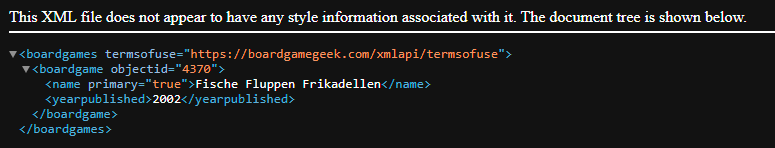
\includegraphics[width=1\textwidth]{graphics/Search_API.png}
    \caption{Ergebnis der `/xmlapi/search`-Funktion bei Suchterm Frika.}
    \label{fig:Search_API}
\end{figure}
\subsubsection{Detaillierte Spielinformationen}
Der zweite Endpunkt ist die „/xmlapi/boardgame/<gameid>“-Funktion und dient dazu,
detaillierte Informationen zu einem Brettspiel zu erhalten. Nutzer könnten hier noch einige weitere Parameter mitgeben um spezifische Informationen zu erhalten, jedoch ist dies in unserem Projekt nicht notwendig, da die Ergebnisse schon detailliert genug sind.
Die \texttt{gameId} ist hierbei der Input, ist gleichzusetzen mit der objectId und kann aus des oben erhaltenen Ergebnisses der Suchfunktion entnommen werden.
Die detaillierten Spielinformationen enthalten folgende Informationen:
\begin{table}[H]
    \centering
    \begin{tabular}{|c|c|}
        \hline
        \textbf{Name} & \textbf{Formattyp} \\
        \hline
        \texttt{objectId} & \texttt{String} \\
        \texttt{yearPublished} & \texttt{String} \\
        \texttt{minPlayers} & \texttt{String} \\
        \texttt{maxPlayers} & \texttt{String} \\
        \texttt{playingTime} & \texttt{String} \\
        \texttt{minPlayTime} & \texttt{String} \\
        \texttt{maxPlayTime} & \texttt{String} \\
        \texttt{age} & \texttt{String} \\
        \texttt{description} & \texttt{String} \\
        \texttt{name} & \texttt{Array (String)} \\
        \texttt{publisher} & \texttt{Array (String)} \\
        \texttt{averageWeight} & \texttt{String} \\
        \texttt{averageRating} & \texttt{String} \\
        \texttt{thumbnail} & \texttt{String (URL to thumbnail image)} \\
        \texttt{usersRated} & \texttt{String} \\
        \hline
    \end{tabular}
    \caption{Die zurückgegebenen detaillierten Informationen.}
    \label{tab:boardgame_properties}
\end{table}
Es ist zu erkennen, dass der Name und der Publisher Arrays sind. Dies lässt sich darauf zurückführen, dass es mehrere Namen für dasselbe Spiel gibt (teilweise auch in anderen Sprachen) und mehrere Entwicklet beteiligt sein können.
\subsubsection{Game of the Day}
Der dritte Endpunkt im Bunde ist die `xmlapi2/hotoverall`-Funktion. Sie gibt die top 50 Spiele mit besonders guter Bewertung und Beliebtheit zurück.
Dabei werden genau fünf unterschiedliche Informationen aufgeführt:
\setlength{\itemsep}{-1pt}
\setlength{\parskip}{-1pt}
\begin{itemize}
    \item id: String (objectId von vorher earlier)
    \item rank: String (Ranking Position der Top 50 Spiele)
    \item thumbnail: String (URL to thumbnail image)
    \item name:  String        
    \item yearpublished 
\end{itemize}
Im Anschluss kann ebenfalls mit der ObjectId eine Anfrage für detaillierte Informationen gestartet werden. 
Einsatz findet dieses Verfahren wenn mit einem Klick das Spiel des Tages ausgewählt wird und somit die zurückgegebene ObjectId auf die Infopage
weitergeleitet wird. Somit konnte eine weitere Seite wiederverwendet werden und zudem ein neues Feature für die App ermöglicht. 
\subsection{MongoDB API}
In diesem Teil wird nur der externe Aufruf auf den selbsterstellten MongoDB \ac{API}-Endpunkt behandelt. 
Der interne Aufbau der MongoDB wird in der Beschreibung der App aufgeführt. Es gibt insgesamt drei Zugriffsmethoden für jede Collection auf die MongoDB: 
\begin{itemize}
    \item \texttt{searchGamesWishlist()}
    \item \texttt{searchGamesInventory()}
    \item \texttt{addToWishlist(gameData)}
    \item \texttt{addToInventory(gameData)}
    \item \texttt{removeFromWishlist(objectId)}
    \item \texttt{removeFromInventory(objectId)}
\end{itemize}
Die GET-Methode, bezieht sich auf den HTTP Endpoint
\texttt{http://localhost:8999/wishlisht} bzw. \texttt{/inventory} und liefert eine Liste aus JSON-Elementen zurück.
Für das Hinzufügen von Brettspielen wird die HTTPClient Methode POST benutzt und die gameData übergeben, wobei Gamedata ein Objekt des Modells Boardgame.ts ist. 
Dieses Objekt wird dann in eine JSON Form in die ausgewählte Collection hinzugefügt. Bei der Entfernung eines Spiels wird als Parameter die ObjectId des Spiels übergeben.
Dieser einzigartige Klassifikator sorgt dafür, dass wenn ein Spiel in der Collection enthalten ist, dass diese ObjectId als Klassifikator verwendet, wird dieses Brettspiel entfernt.
Des Weiteren ist dies aus Effizienzgründen vorteilhaft, da kein komplettes Objekt übergeben wird, geparsed werden muss und schlussendlich verglichen. Eine Überprüfung kann direkt stattfinden.
\begin{center}
    \begin{lstlisting}[caption={Löschaufruf der MongoDB API}, label=lst:jscode]
    this.http.delete(`${this.inventoryUrl}/${objectId}`)
\end{lstlisting}
\end{center}


\subsection{Verwendung der APIs im Projekt selbst}
Die Definition der Methoden zum Aufrufen der \ac{API}-Endpunkte ist in der Datei \\\texttt{board-game.service.ts} des \texttt{services}-Ordner zu finden.
Dazu wird das HTTPClient Modul importiert und es wird ein htttp.get Aufruf mit den jeweiligen Parametern durchgeführt. Da das Ergebnis in Form einer XML-Datei vorliegt und es vorteilhafter ist mit einem JSON-Format zu arbeiten, wird zu Beginn eine Transformation des Formats in die JSON-Form durchgeführt.
Dies geschieht konkret durch das importierte Modul „xml2json“. \bigskip 

Die vorliegende JSON-Datei kann nun dem Modell \texttt{game.ts}, \texttt{boardgame.ts} oder \\\texttt{randomtopgame.ts} zugewiesen werden. Also eine Initialisierung einer Liste von Objekten dieser Modelle basierend auf dem spezifischen \ac{API}-Aufruf.
Im Folgenden wird dann ein Array als \texttt{return}-Element der Funktion definiert. Dies ermöglicht es erstmalig ein subscribe auf die Funktion zu legen und auf der benötigten Seite anzuzeigen. \bigskip 

Die konkrete Verwendung der APIs ist auf den folgenden Pages ist wie folgt:

\begin{itemize}
    \setlength{\itemsep}{-1pt}
    \setlength{\parskip}{-1pt}
    \item Homepage
        \begin{itemize}
        \item Game of the Day mit `xmlapi2/hotoverall`-Funktion
        \end{itemize}
    \item Searchpage
        \begin{itemize}
        \item Suchfunktion mit `/xmlapi/search`-Funktion
        \end{itemize}
    \item Inventory, Wishlist
        \begin{itemize}
        \item MongoDB GET mit ``http://localhost:8999/inventory/''-Funktion 
        \end{itemize}
    \item Infopage
    \begin{itemize}
    \item Detaillierte Spielinformationen mit `/xmlapi/boardgame/<gameid>`-Funktion 
    \item MongoDB mit ``http://localhost:8999/inventory?objectId''-DELETE Funktion
    \item MongoDB mit ``http://localhost:8999/inventory?gameData''-ADD Funktion
    \item MongoDB mit ``http://localhost:8999/wishlisht?objectId''-DELETE Funktion
    \item MongoDB mit ``http://localhost:8999/wishlisht?gameData''-ADD Funktion
    \end{itemize}

\end{itemize}
\section{Beschreibung der Docker-Umgebung}
In der Docker-Umgebung werden vier Services für die Anwendung rund um die Verwaltung
von Brettspielen definiert. Diese Anwendung verwendet Docker, um die Entwicklung und
Bereitstellung zu vereinfachen und zu standardisieren. Die Konfiguration umfasst vier
Hauptdienste: MongoDB-Datenbank, Mongo-Express für die Datenbankverwaltung, einen
Server für die Kommunikation zwischen Frontend und Datenbank sowie einen Proxy-Server
für den Zugriff auf die BGG (BoardGameGeek) API, um CORS-Probleme zu vermeiden.
\subsection{MongoDB-Datenbank}
Dieser Dienst verwendet das offizielle
MongoDB-Image und ist so konfiguriert, dass er automatisch neu startet, falls es zu einem
Fehler kommt.
Die Umgebungsvariablen \\\texttt{MONGO\_INITDB\_ROOT\_USERNAME} und
\texttt{MONGO\_INITDB\_ROOT\_PASSWORD} sind auf \texttt{admin} gesetzt, wodurch die Anmeldedaten für
den Datenbankzugriff definiert sind. Der Dienst nutzt ein Volume \texttt{MONGO\_DATA}, um Daten
dauerhaft zu speichern und macht den Standard-MongoDB-Port 27017 für andere Dienste
zugänglich.
\subsection{Mongo-Express}
Als webbasiertes Verwaltungstool für
MongoDB erleichtert Mongo-Express die Verwaltung der Datenbank über einen Webbrowser.
Es ist ebenfalls so eingestellt, dass es immer neu startet und verwendet die gleichen
Anmeldeinformationen wie die MongoDB. Dieser Dienst hängt von \texttt{mongo\_boardgame} ab
und kommuniziert über den internen Netzwerknamen. Mongo-Express ist über den Port 9001
zugänglich.
\subsection{Server}
Dieser Dienst baut einen Server aus einem Dockerfile, das sich im Verzeichnis
\\\texttt{../assignment\_gruppe\_2\_server} befindet. Der Server dient als Schnittstelle zwischen dem
Frontend und der MongoDB-Datenbank. Er ist über den Port 8999 erreichbar.
\subsection{Proxy-Server}
Der Proxy-Server ermöglicht den sicheren Zugriff auf externe
APIs, in diesem Fall die BGG \ac{API}, entweder die xmlapi oder die xmlapi2
\href{https://api.geekdo.com/xmlapi2}{dieser Webseite} (Doku \href{https://boardgamegeek.com/wiki/page/BGG_XML_API2}{hier} abrufbar).
Der Container wird aus einem Dockerfile gebaut, welches im Verzeichnis des Proxy-Servers liegt. Der
Dienst ist über den Port 8888 erreichbar und so konfiguriert, dass er stets neu startet.
\subsection{Volumes}
Ein definiertes Volume \texttt{MONGO\_DATA} wird verwendet, um die Datenbankdaten
dauerhaft zu speichern und sicherzustellen, dass diese über den Neustart von Containern
hinweg erhalten bleiben.
\subsection{Zusammenfassung}
Zusammenfassend stellt dieses Docker Compose-Projekt eine vollständige Umgebung für die
Entwicklung und Bereitstellung der Brettspiel-App bereit. Es automatisiert die Konfiguration
und Verwaltung von Diensten, die für die Speicherung von Daten, die Verwaltung der
Datenbank, die Kommunikation mit dem Frontend und den sicheren Zugriff auf externe APIs
erforderlich sind. Die Server sind intern so konfiguriert das sie vollen Zugriff zulassen, sodass
keine CORS-Probleme auftreten auch durch das Ansprechen auf dem lokalen Gerät durch den
Emulator.
\section{Beschreibung des Proxys und des externen Routings}
Der Docker-Container mit dem Proxy ist zuständig für die Kommunikation zwischen der App
und der externen \ac{API}. Dies ist notwendig da der Server hinter der \ac{API} eine direkte Anfrage
nicht akzeptiert und CORS-Probleme auftreten. Deshalb hilft der Proxyserver, indem dieser
seine Herkunft verschleiert und Anfragen von der App an die \ac{API} weiterleitet. Dabei gibt es
drei Suchanfragen, welche die App verwendet:
\begin{itemize}
    \item \href{https://api.geekdo.com/xmlapi2/hotoverall}{Diese Anfrage} gibt in XML-Format die 50 bestbewertetsten Brettspiele zurück.
    \item \href{https://api.geekdo.com/xmlapi/search?search=}{Diese Anfrage} kann nach Spielen suchen, indem hinter den \texttt{search}-Teil der URL ein oder mehrere Buchstaben bzw. Worte gesetzt werden, wodurch nach einem Spiel gesucht werden kann. Es wird eine XML-Datei zurückgegeben, die alle Brettspiele enthält, auf welche die Beschreibung des Searchstring zutrifft. Je ungenauer die Anfrage gestellt wird, desto länger wird auf die Rückmeldung des Servers gewartet, um alle Spiele darzustellen. Ein Beispiel kann \href{https://api.geekdo.com/xmlapi/search?search=to}{hier} geöffnet werden.
    \item Mit \href{https://api.geekdo.com/xmlapi/boardgame/1&stats=1} {dieser Anfrage} können alle für die App wichtigen Informationen eines Brettspiels aufgerufen werden (inklusive der Statistiken und Bewertungen). Für das Aufrufen dieser Seite ist die ID des Objektes von höchster Relevanz, in dem Beispieladresse sieht man die erste 1, welche auf die ID des Brettspiels verweist. Diese wird durch die ID des gesuchten Spiels ersetzt. Diese ID wird genommen von der Auswahl von den durch die Suche gefundenen Daten oder den Daten, die in Wishlist/Inventory gespeichert sind.
\end{itemize}
Das Routing funktioniert ausgehend von der boardgame.service.ts dort wird vom System
unterschieden ob momentan von einem Emulator/einem Mobilgerät \texttt{http://10.0.2.2:\dots} oder über den
Lokalhost \texttt{http://localhost:\dots} kommuniziert wird. Dadurch werden die gesamten Pfade an das
Herkunftssystem angepasst. Eine Anfrage an den Proxy wird dabei mit \texttt{/redirect} durchgeführt. Der
Proxy hört darauf wenn er angesprochen wird und entfernt das /redirect aus dem Suchstring um die
Anfrage an die BGG-API weiterzuleiten. Dabei wird der Proxy als Übermittler verwendet und dieser
gibt beidseitig die Ergebnisse der Anfragen weiter und ermöglicht dadurch eine indirekte
Kommunikation zwischen Applikation und API-Server.
\section{Anleitung zum Starten der Applikation}
Zuerst muss von Git das gesamte Asignment-Gruppe-2 Projekt auf das lokale Gerät gezogen werden.
Auf diesem lokalen Gerät werden einige Bedingungen vorausgesetzt:
\begin{enumerate}
    \item Docker muss bereits existieren.
    \item \ac{VM} müssen im \ac{BIOS} aktiviert sein.
    \item Für das Starten der emulierten App auf einem emulierten Endgerät wird ein Emulator vorausgesetzt.
    \item Eine Internetverbindung ist erforderlich.
\end{enumerate}
Wenn all diese Bedingungen erfüllt sind und das Projekt vorliegt, muss eine Kommandozeile/Terminal
(mit Adminrechten) gestartet werden.
\begin{enumerate}
    \item Navigiere auf das Projekt: \\\texttt{cd <derPfad>/assignment-gruppe-2}.
    \item Installiere die relevanten Paketmodule für die Node-Umgebung: \texttt{npm install}.
    \item Navigiere auf das Docker-Compose um alle notwenigen Container zu starten: \\\texttt{cd <derPfad>/assignment-gruppe-2/assignment\_gruppe\_2\_mongo\_DB}.
    \item Führe das Docker-Compose permanent aus um automatisiert die vier Images zu bilden, die für die App benötigt werden: \texttt{docker compose up -d}. Dabei werden die Images gebaut und dann in Docker bereits gestartet, dies sollte für die folgenden Schritte im Terminal oder über eine graphische Ansicht der Docker-Container überprüft werden (siehe Fig. \ref{fig:docker}).
    \item Navigiere zurück auf das Gesamtprojekt: \\\texttt{cd <derPfad>/assignment-gruppe-2}.
    \item Möglichkeit 1: Zum Starten von der Applikation im Browser nutze: \texttt{ionic serve}. Dies sollte ein Fenster öffnen mit \url{http://localhost:8100/home}, welches die App anzeigt. Für eine sinnvolle Anzeige lohnt sich das Aktivieren der Mobilgerätesicht.
    \item Möglichkeit 2: Zum Starten der App auf einem emulierten Endgerät nutze, öffne ein Emulator und starte ein Gerät und spreche es mit dem folgenden Befehl an, um das Spiel auf diesem Gerät zu starten: \\\texttt{ionic cordova run android} (siehe Fig. \ref{fig:emulator}).
\end{enumerate}
\begin{figure}[H]
    \centering
    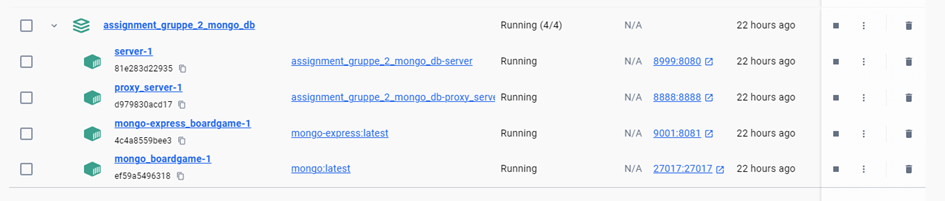
\includegraphics[width=1\textwidth]{graphics/docker.png}
    \caption{Docker-Container nach dem Starten.}
    \label{fig:docker}
\end{figure}
\begin{figure}[H]
    \centering
    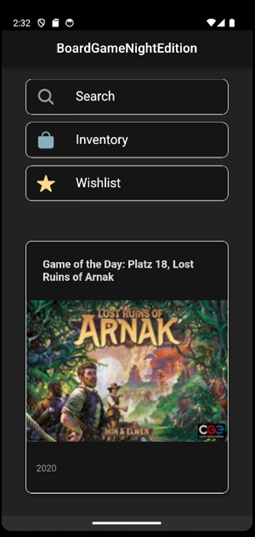
\includegraphics[width=0.35\textwidth]{graphics/emulator.png}
    \caption{Emulator nach dem Starten der App.}
    \label{fig:emulator}
\end{figure}